\subsection{Numeric treatment}

To verify the analysis we compared Eq.\,(\ref{eq:kappa_rT1_lambda4}) against numerical simulation of the measurement circuit using the LTSPICE \footnote{www.linear.com/designtools/software} circuit simulation package.
Figure \ref{Fig:SPICEDiagram} shows a diagram of the model.
We determine the quality factor of the qubit $Q_q$ in two steps.
First we replace the qubit with a voltage source $V_s$ at frequency $\omega$ and probe the resulting current $I_s$.
The ratio $I_s / V_s$ is the admittance $Y_e(\omega)$ of the external measurement circuitry as seen by the qubit.
We then use the fact that, for the transmon qubit, the matrix elements are nearly those of a harmonic oscillator.
For a harmonic system, the coherent states are eigenvectors of the annihilation operator $a$, so loss processes are always in the correspondence limit.
We can therefore compute the damping of the qubit using the classical equation \cite{Esteve:dissipation1986}  \begin{equation}
Q_q = \omega C_q / \Re{Y_e(\omega)}. \label{eq:Q_qAdmittance} \end{equation}

The LTSPICE package easily simulates a given circuit over a range of frequencies, but has somewhat limited capabilities for iterating over circuit element values.
In order to facilitate the design process we have written a driver for LTSPICE in python.
This driver allows the user to programmatically import an existing net list (e.g. one produced by a graphical front-end), override parameter values, and produce a new updated net list which is then analyzed by SPICE.
Combined with a python module for parsing the resulting simulation data, this driver allowed us to easily iterate over several design parameters and analyze the results in a powerful programming environment.

\begin{figure*}
\begin{centering}
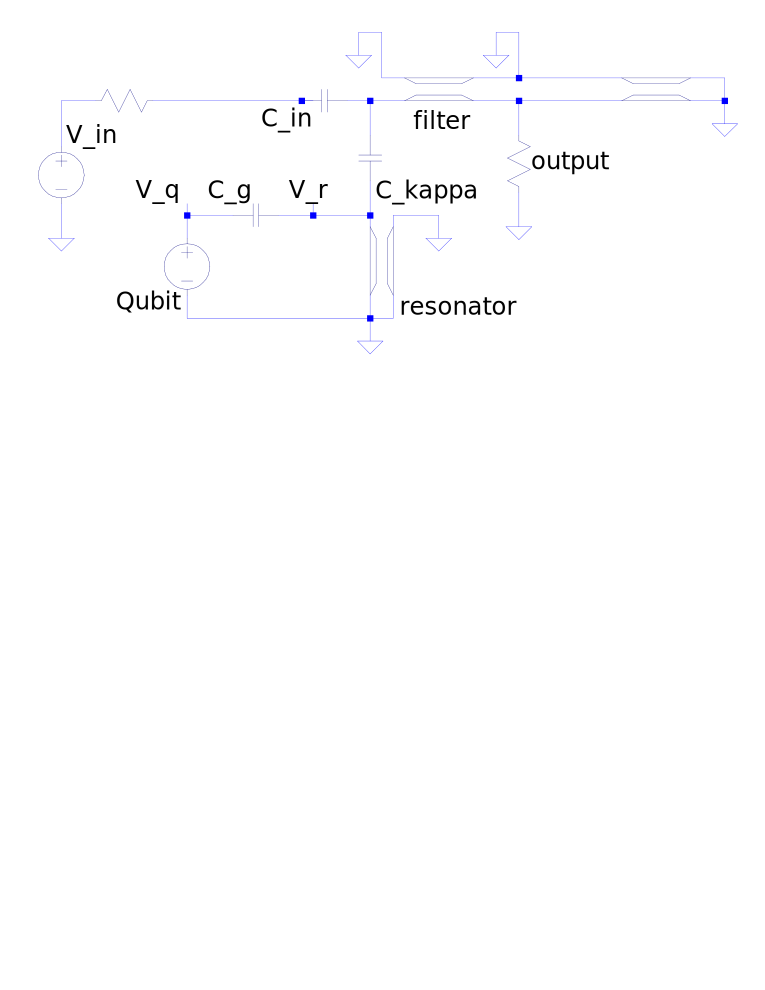
\includegraphics[width=\textwidth]{screenshot_SPICE.pdf}
\par\end{centering}
\caption{Screen capture of the SPICE model. The qubit is replaced by a voltage source which is activated with an ac signal of amplitude $V_s$ at variable frequency $\omega$. The current $I_s$ through the source is probed and the admittance of the external circuit computed as $Y_e(\omega)=I_s / V_s$. Note that the filter $\lambda/4$ transmission line resonator is not drawn to scale; the end which connects to ground is physically shorter than the other section.}
\label{Fig:SPICEDiagram}
\end{figure*}

\subsection{Discussion}

The results of the numerical simulation are compared with the analytic theory in Fig.\,\ref{Fig:purcellTheoryVsNumerical}.
The expected $T_1$ of the qubit is plotted against the qubit-resonator detuning $\Delta$ for a few values of $\kappa_r$ and $Q_F=30$.
Good agreement between the theory and numerics appears for $\left| \Delta \right| \approx 1\,\text{GHz} \text{ to } 0.5\,\text{GHz}$.
For detunings below -1.5\,GHz the analytic formula exceeds the numerics by approximately a factor of 2.
This is probably due to our imperfect assumption that the coupling impedances greatly exceed the resonator impedances.
When $\left| \Delta \right|$ is on the order of $g$ the qubit and resonator modes hybridize.
In this regime the analytic and numerical treatments are both expected to fail because Eq.\,(\ref{eq:Q_qDefinition}) and Eq.\,(\ref{eq:Q_qAdmittance}) both implicitly assume that the qubit mode is well defined apart from the rest of the measurement circuit.
This failure is manifest in the plots near $\Delta=0$ where the predicted qubit $T_1$ becomes smaller than $\kappa_r$.
This is not physical, as the system cannot lose energy faster than the bare leakage rate of the resonator $\kappa_r$.

The predictions shown in Fig\,\ref{Fig:purcellTheoryVsNumerical} indicate that we should be able to preserve the qubit coherence with very aggressive resonator ring-up times.
The curve for $\kappa_r^{-1} = 11\,\text{ns}$ has a $T_1$ limit of $100\,\mu\text{s}$ at $\left| \Delta \right| = 1\,\text{GHz}$ and $1000\,\mu\,\text{s}$ at $\left| \Delta \right| = 1.5\,\text{GHz}$.
These are modest detuning values typical of real experiments. Current best $T_1$ values for planar transmon qubits are near $60\,\mu\text{s}$ with typical values around $20\text{--}40\,\mu\text{s}$.
With the measurement circuit bringing in a decoherence channel at $1000\,\mu\text{s}$ a qubit with internal $T_1$ of $60\,\mu\text{s}$ would be degraded by only 5\%.

Because the $T_1$ imposed by the measurement circuit varies by several orders of magnitude with varying $\Delta$, it should be possible to use the measurement circuit as a reset.
By dynamically tuning the qubit close to the measurement resonator and filter, the $T_1$ of the would be lowered, forcing the qubit to go to $\ket{0}$ with high probability after several decay time constants.
This could be particularly useful in removing ``leakage'' processes in which the qubit has erroneously gone to state $\ket{2}$.

\begin{figure}
\begin{centering}
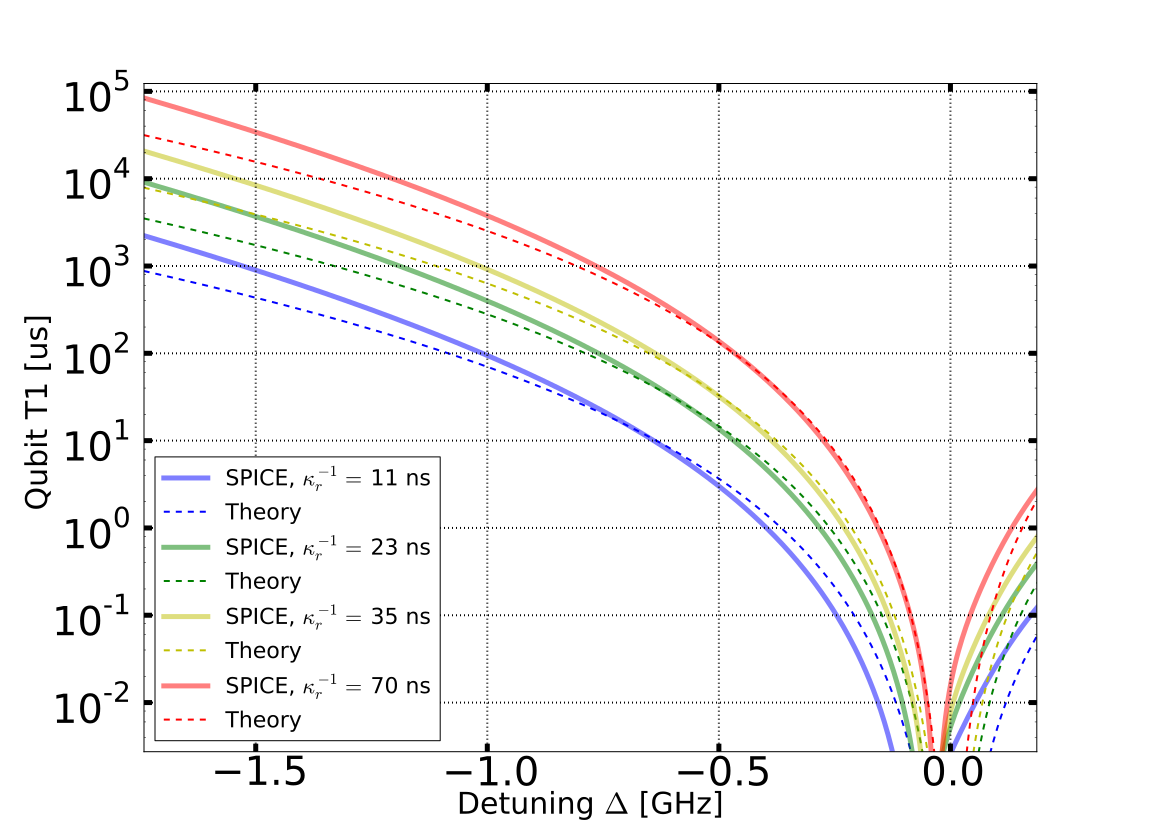
\includegraphics[width=\textwidth]{purcell_theory_vs_numerical.pdf}
\par\end{centering}
\caption{Qubit $T_1$ imposed by the measurement circuit versus qubit-resonator detuning for several values of the resonator decay time. The filter quality factor is $Q_F=30$.}
\label{Fig:purcellTheoryVsNumerical}
\end{figure}

